\chapter{数据同步与平滑机制的引入}
\section{初步运行测试}
经过第四章中设计与实现的内容后,我们得到了一个可以连接仿真机和图像生成器并转换双方指令的数据交换子系统。
为测试系统在真实FFS环境下的表现,需要去到飞行训练基地接入专业设备进行初步的功能测试。
\subsection{测试环境}
为使用真实仿真机设备,我们去到南方航空珠海训练基地。此处是亚洲最大,机型最全的模拟飞行训练基地,共拥有28台民航局运输司认证的最高D等级FFS,每年有超过7000名飞行员在此训练,是名副其实的中国民航飞行员培养摇篮。
\par
该测试环境中各设备布置方式如图\ref{testenv}所示。虚拟仿真机需要配置两张网卡,一张通过交换机连接仿真机,另一张通过交换机连接三台图像生成器。
三台图像生成器各自连接一台投影仪才能实现对模拟座舱前方球幕的融合投影。
\begin{figure}[h!]
    \begin{center}
        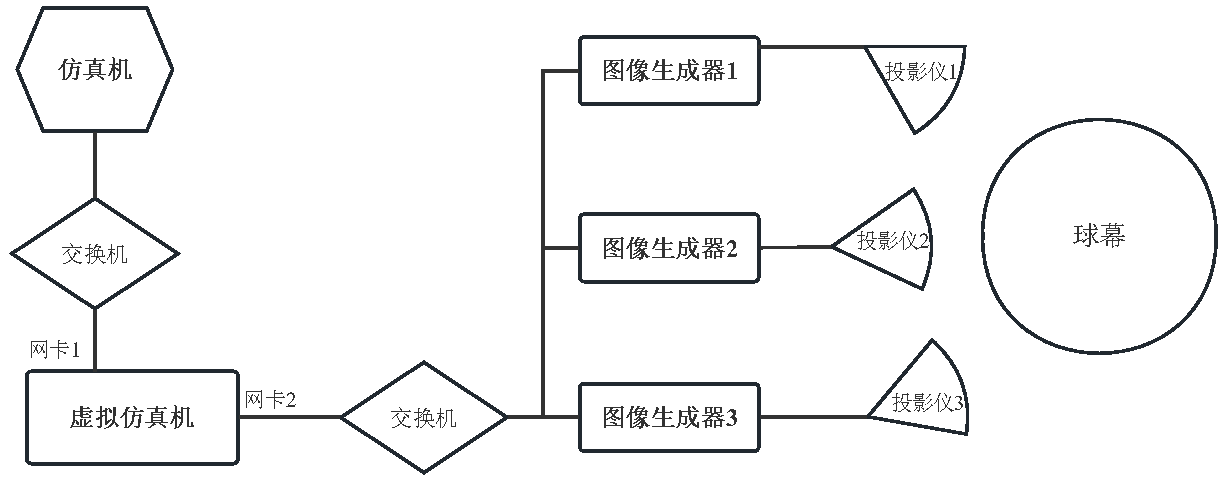
\includegraphics[width=\textwidth]{pictures/testenv.pdf}
        \caption{测试环境设备布置}
        \label{testenv}
    \end{center}
\end{figure}
\par
此环境下虚拟仿真机运行于一台机器上,三台图像生成器运行在配置完全相同的三台机器上,它们通过网线连接交换机。
为了顺利运行视景系统,运行设备上需要配置系统运行的软件环境,详细信息如表\ref{devsoft}所示。
虚拟仿真机和图像生成器两方都需要C++与Python的运行环境,且双方需要通过Tbuspp插件沟通。
在虚拟仿真机中,需要使用WinPcap软件侦听流经网卡的数据包。测试环境部署配置完成后应当能保证系统不会因为软件环境问题无法运行。

\begin{table}[h!]
    \begin{center}
        \caption{软件配置表}
        \label{devsoft}
        \renewcommand\arraystretch{1.5}
        \begin{tabularx}{0.8\textwidth}{ 
             >{\centering\arraybackslash\hsize=.5\hsize\linewidth=\hsize}X 
             >{\centering\arraybackslash\hsize=\hsize\linewidth=\hsize}X 
             }
             \hline
            \textbf{配置项 } & \textbf{详情}\\
             \hline
             C++运行环境 & VS\_C++\_MSVC\\
           
             Python运行环境 & Python\thinspace 3.10\\
             
             底层网络访问 & WinpCap\thinspace v4.1.3\\
            
             服务网格 & Tbuspp \thinspace 0.6.0\\
             \hline
            \end{tabularx}
    \end{center}
\end{table}
\par
在硬件配置方面,运行图像生成器的机器基本配备最新且性能最强的配件,保障渲染帧率能跟上仿真机产生数据的频率。测试环境下的具体硬件配置信息如表\ref{ffshard}所示。
测试环境中的网络完全隔绝外部网络,网络环境非常良好,网络时延在1ms内,网络抖动几乎为0。也意味着如果测试中出现问题,网络环境并不是一个首先需要考虑的因素。

\subsection{功能测试}
对于本数据交换子系统的功能测试依照指令代号进行。第三章中提到目前已经验证了21种仿真机指令,我们让飞行员和教练员在模拟座舱中进行操作依次产生这些指令,
如果投影画面产生了对应指令代号的变化,则说明数据交换子系统对于该类指令的接收、转换、发送、分配使用的过程顺利,可以通过测试。
表\ref{testcase}给出了对于仿真机指令代号为21H指令的测试用例,该指令负责控制飞机的位置和姿态,其他种类指令的测试用例与此表类似。
\clearpage
\begin{table}[h!]
    \begin{center}
        \caption{硬件配置表}
        \label{ffshard}
        \renewcommand\arraystretch{1.5}
        \begin{tabularx}{\textwidth}{ 
             >{\centering\arraybackslash\hsize=.4\hsize\linewidth=\hsize}X 
             >{\centering\arraybackslash\hsize=.4\hsize\linewidth=\hsize}X 
             >{\centering\arraybackslash\hsize=\hsize\linewidth=\hsize}X 
             }
             \hline
            \textbf{设备} & \textbf{配置项} & \textbf{详情}\\         
             \hline
             & CPU & Intel® Core™ i9-12900K Processor\\
           
             & GPU & NVIDIA RTX A6000\\
             
             图像生成器 & 内存 & 64GB\\
            
             & 硬盘 & 8TB\\
             
             & 系统 & Windows 10 专业版 21H2\\
             \hline
             & CPU & Intel® Core™ i9-12900K Processor\\
           
             & GPU & Intel® UHD Graphics 770\\
             
             虚拟仿真机 & 内存 & 32GB\\
            
             & 硬盘 & 2TB\\
             
             & 系统 & Windows 10 专业版 21H2\\
             \hline
             
            \end{tabularx}
    \end{center}
\end{table}
\begin{table}[h!]
    \begin{center}
        \caption{控制指令21H测试用例}
        \label{testcase}
        \renewcommand\arraystretch{1.5}
        \begin{tabularx}{0.8\textwidth}{ 
             >{\centering\arraybackslash\hsize=.2\hsize\linewidth=\hsize}X 
             >{\raggedright\arraybackslash\hsize=.8\hsize\linewidth=\hsize}X 
             }
             \hline
            \textbf{ID } & \textbf{TC1}\\
             \hline
             \textbf{测试名称} & 仿真机21H指令控制测试\\
             \hline
             \textbf{待测功能} & 图像生成器能接收并使用转换后的21H指令。\\
             \hline
             \textbf{测试步骤} & 1.飞行员通过操纵杆让飞机运动。\par 2.仿真机生成21H指令。\par 3.虚拟仿真机转换其为自定义指令。\par 4.图像生成器收到指令分配给对应处理逻辑。  \\
             \hline
             \textbf{预期结果} & 投影画面中的飞机按飞行员的操作运动。\\
             \hline
            \end{tabularx}
    \end{center}
\end{table}
\par
图\ref{21test}展示了投影画面中的飞机根据飞行控制指令沿跑道起飞的过程。证明数据交换子系统对该指令的处理流程通过测试。

\par
图\ref{todtest}展示了投影画面对时间变换指令的响应效果。模拟场景中精确到一天中的每一分钟都可以由时间变换指令控制,
图中是将时间调整到黄昏时分的环境效果。指令被正确应用,数据交换子系统对时间变换指令的处理流程通过测试。
\clearpage
\begin{figure}[h!]
    \begin{center}
        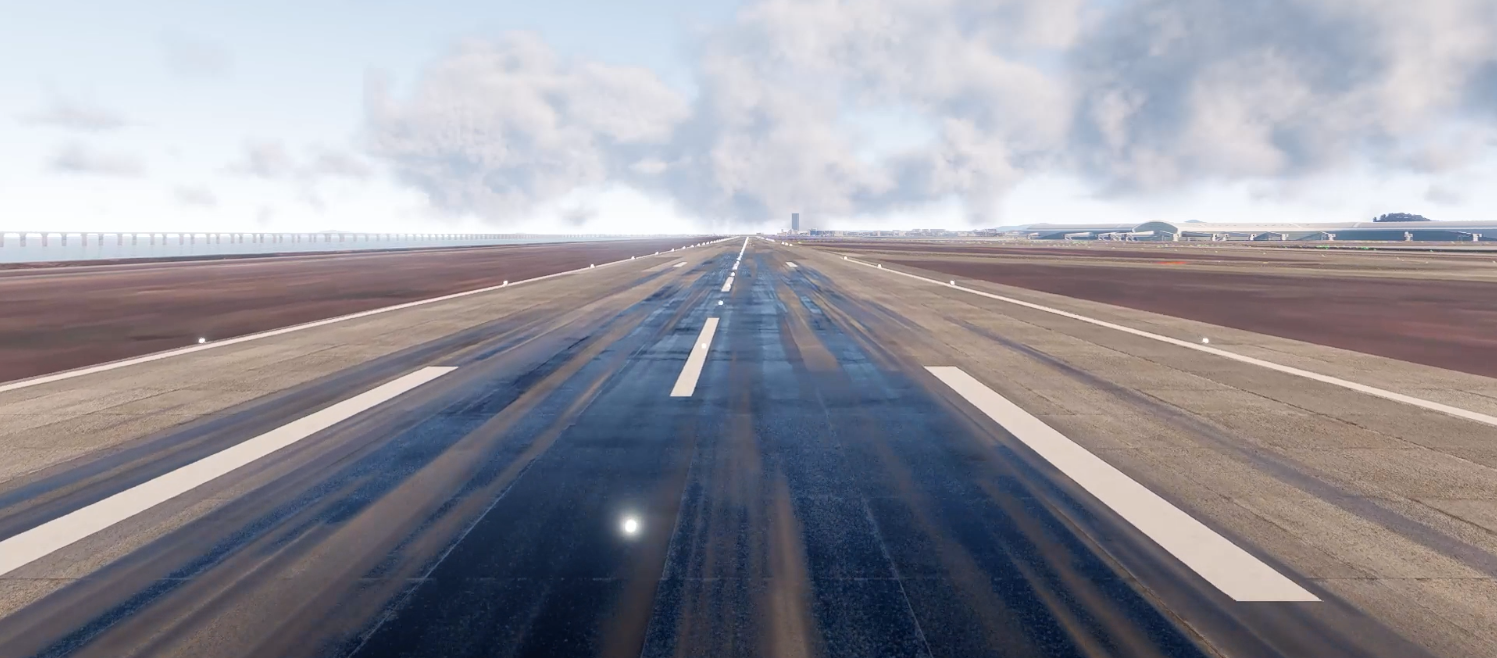
\includegraphics[width=.9\textwidth]{pictures/firstcamera.png}
        \caption{飞行控制指令测试结果}
        \label{21test}
    \end{center}
\end{figure}
\begin{figure}[h!]
    \begin{center}
        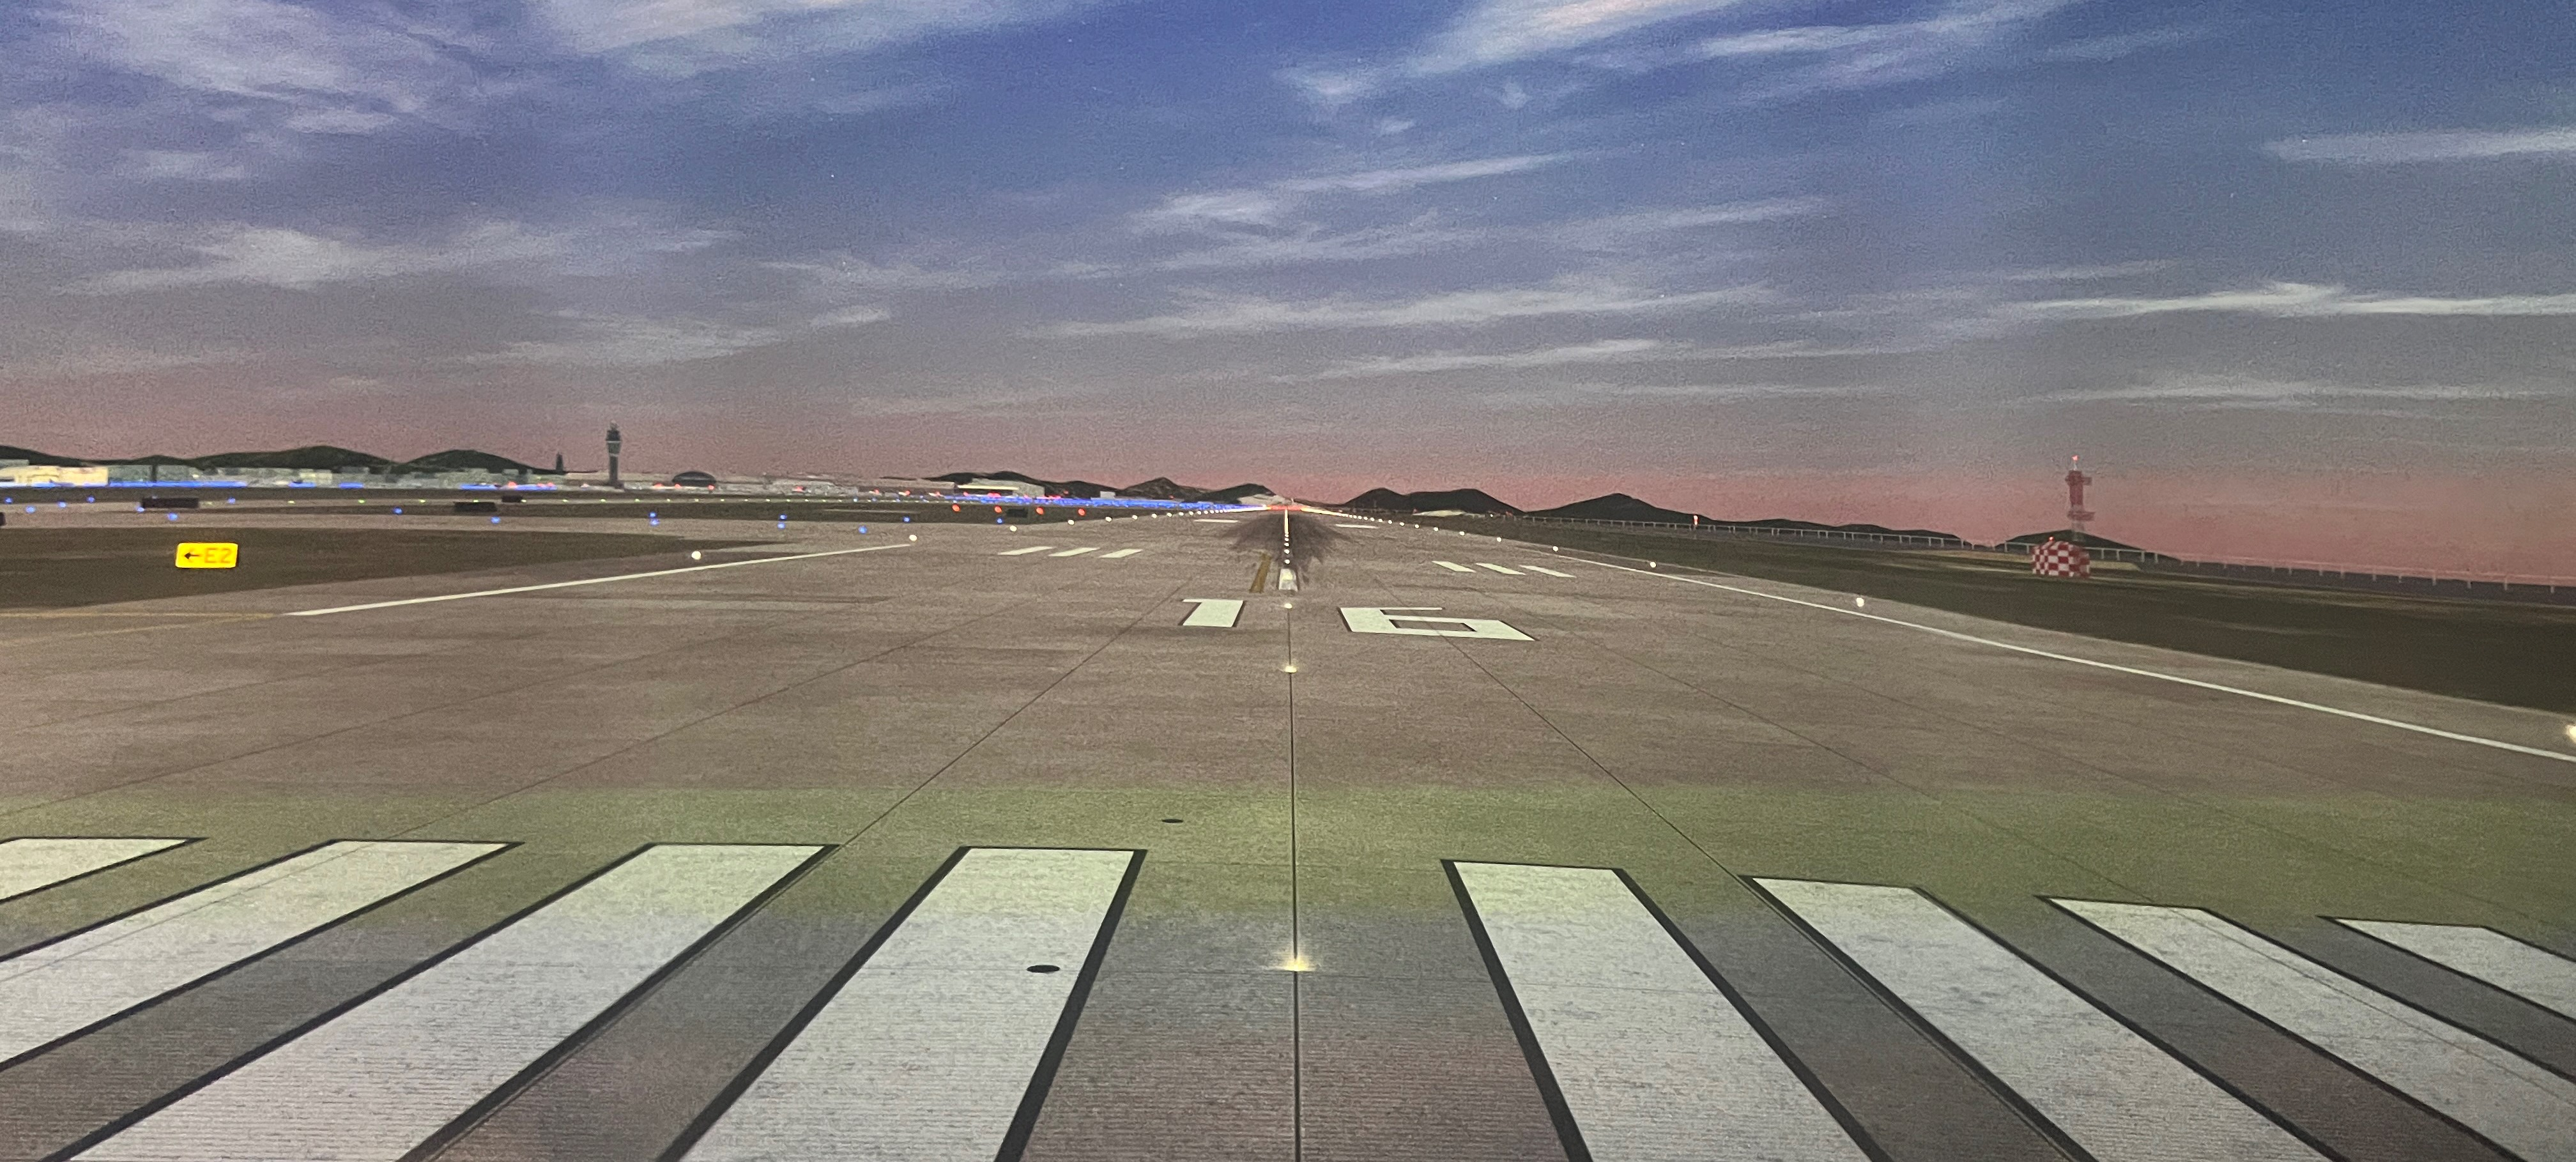
\includegraphics[width=.9\textwidth]{pictures/todtest.jpg}
        \caption{时间变换指令测试结果}
        \label{todtest}
    \end{center}
\end{figure}
\par
图\ref{lighttest}展示了投影画面对灯光控制指令的响应效果。飞机身上诸如滑行灯、机翼灯、防撞灯等多种灯光的开关控制均由灯光指令控制。
图中是飞机在夜间开启滑行灯后的视景效果。指令可以正确应用,数据交换子系统对灯光指令的处理流程通过测试。
\par
图\ref{snowtest}展示了投影画面对天气控制指令的响应效果。飞行过程中的雨雪天气及等级都由天气指令控制,图中展示了视景中大雪天气的效果,
视野中不仅有雪花的加入,能见度也大大降低。指令被正确应用,数据交换子系统对天气指令的处理流程通过测试。
\clearpage
\begin{figure}[h!]
    \begin{center}
        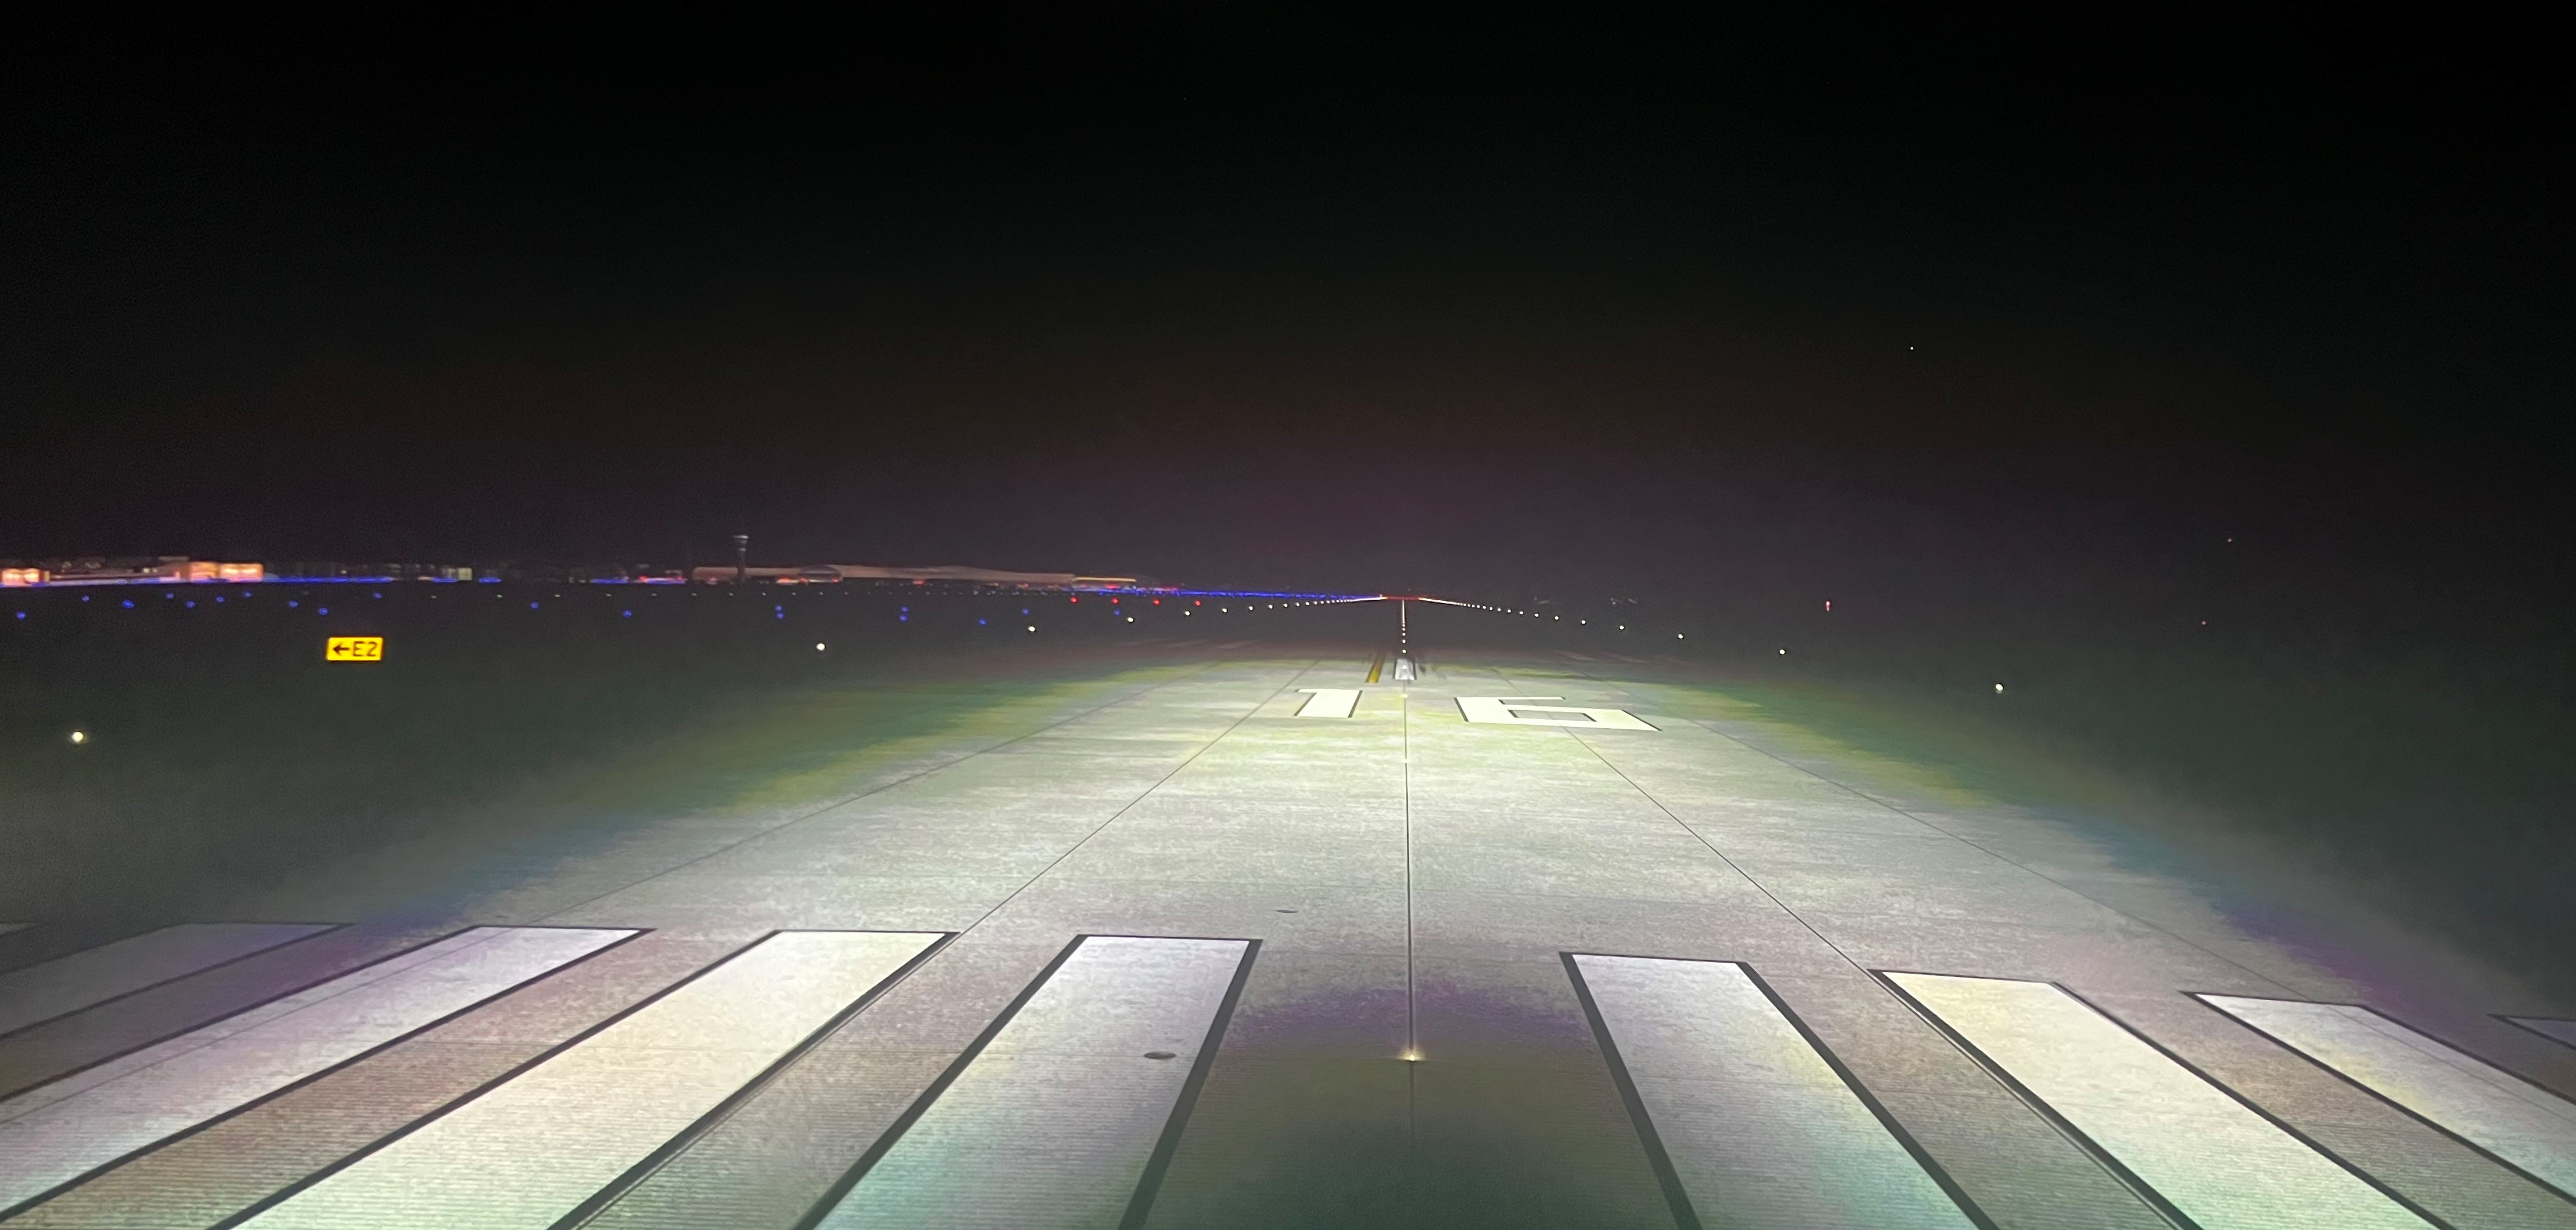
\includegraphics[width=.9\textwidth]{pictures/lighttest.jpg}
        \caption{灯光指令测试结果}
        \label{lighttest}
    \end{center}
\end{figure}
\begin{figure}[h!]
    \begin{center}
        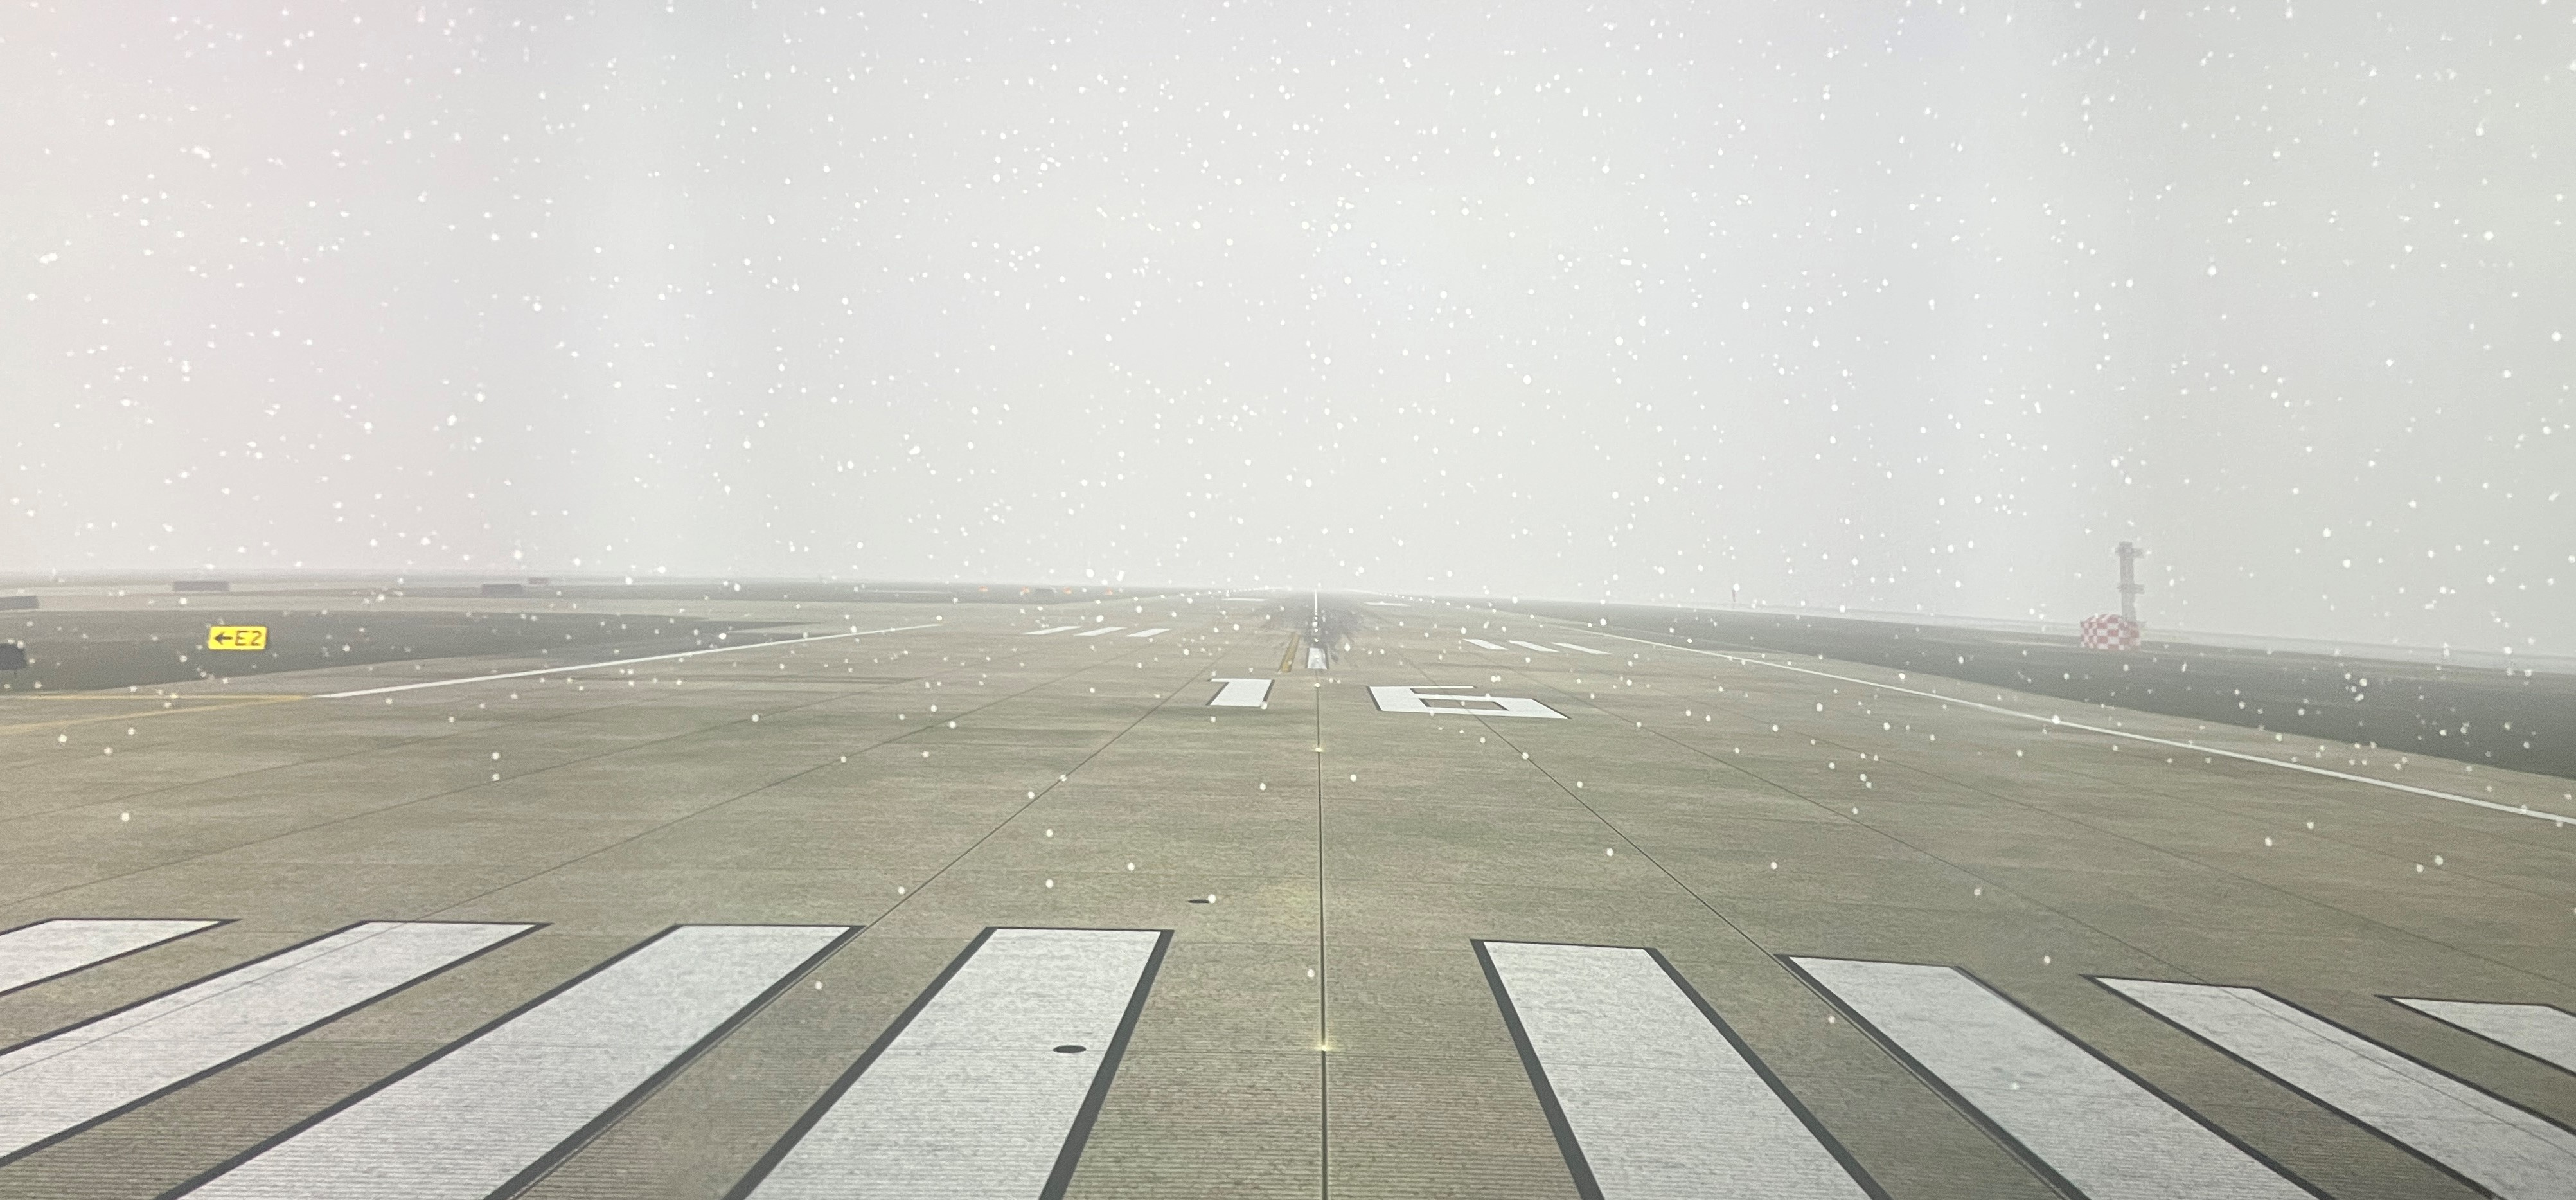
\includegraphics[width=.9\textwidth]{pictures/snowtest.jpg}
        \caption{天气指令测试结果}
        \label{snowtest}
    \end{center}
\end{figure}
\par
当然已通过验证的仿真机指令远不止这些,此处不再逐一列举测试情况。
飞行过程中会产生一些需送回仿真机的反馈指令,比如飞机在起飞和降落过程中会持续检测三个起落架的离地高度。
测试时我们对比了图像生成器构建的自定义指令与从仿真机侧捕获到的仿真机指令中的内容。
表\ref{fbcomp}展示了两方数据的对比结果,仿真机对于高度使用的单位是0.5mm,经换算后与自定义指令一致。
说明数据交换子系统可以正确处理该反馈指令。
\begin{table}[h!]
    \begin{center}
        \caption{反馈信息对比}
        \label{fbcomp}
        \renewcommand\arraystretch{1.5}
        \begin{tabularx}{0.8\textwidth}{ 
             |>{\centering\arraybackslash\hsize=.7\hsize\linewidth=\hsize}X 
             |>{\centering\arraybackslash\hsize=1.15\hsize\linewidth=\hsize}X 
             |>{\centering\arraybackslash\hsize=1.15\hsize\linewidth=\hsize}X
             |
             }
             \hline 
            \textbf{起落架编号} & \textbf{自定义指令} & \textbf{仿真机指令}\\   
             \hline
             1 & 3.822m & 7644\\
             \hline
             2 & 3.787m & 7574\\     
             \hline
             3 & 3.787m & 7574\\
             \hline 
             ...& ... & ...\\
             \hline 
             1 & 40.031m & 80062\\
             \hline 
             2 & 39.914m & 79828\\
             \hline 
             3 & 39.912m & 79824\\
             \hline  
            \end{tabularx}
    \end{center}
\end{table}

\section{数据同步机制}
\subsection{问题分析}
本次测试中同样发现了一些问题。
最具代表性的问题如图\ref{tear}红框中所示,发现在飞行的过程中融合投影的图像中存在撕裂现象。
此处说的图像撕裂并非传统的同一个显示设备的图像上下两部分的撕裂,因为采用了投影仪垂直同步也不会产生这种撕裂。
此时的撕裂是在两台投影仪的交界处存在左右两部分撕裂,即两台设备各自渲染的部分图像并不能完美拼接在一起。
且就整体画面而言,偶尔会出现肉眼可观察的顿挫现象,即存在跳帧的问题。
\begin{figure}[h!]
    \begin{center}
        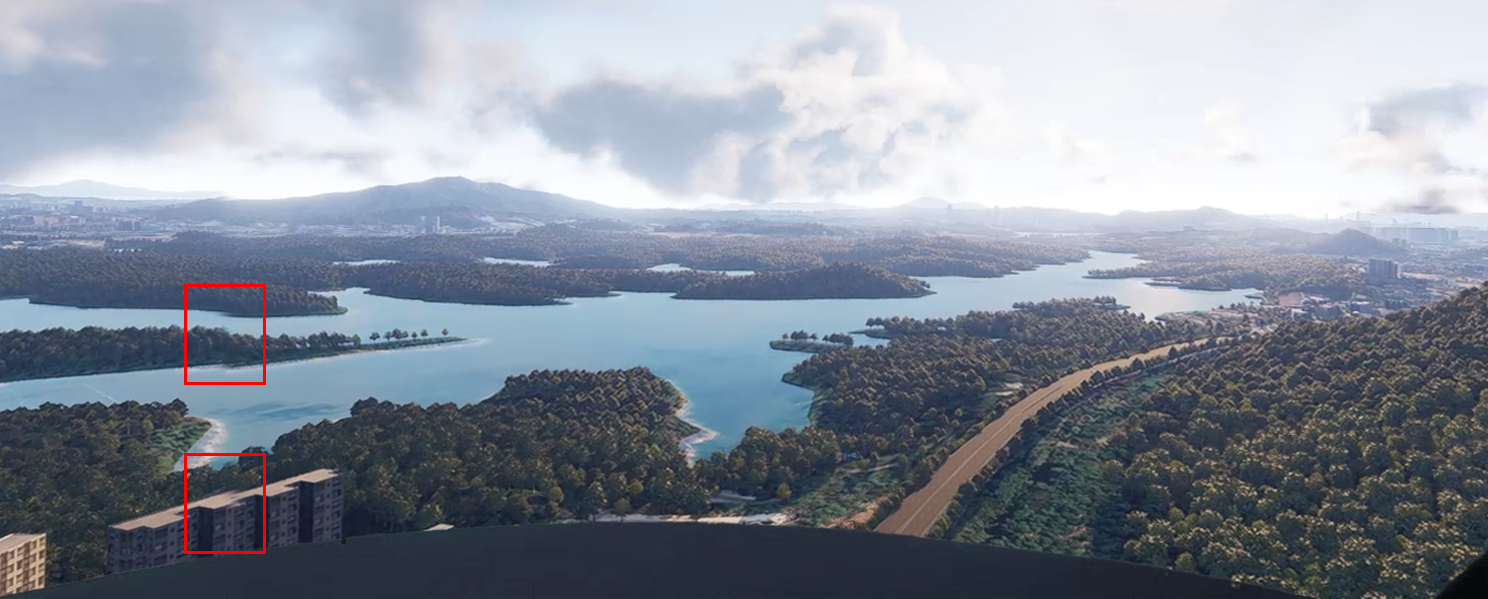
\includegraphics[width=\textwidth]{pictures/tearmark.png}
        \caption{画面撕裂情况}
        \label{tear}
    \end{center}
\end{figure}
\par
对于此现象首先考虑是否投影图像本身就无法拼接,即投影仪校准或多台图像生成器各自渲染时的投影矩阵存在问题,但比较明确的是在飞机静止时并不会出现如上的画面撕裂问题,
这证明并非图像本身无法拼接。由此便仅有一种可能性,便是多台投影仪的投影图像并非同一帧的内容,两侧的图像间产生了差距所以不能拼接。
图\ref{tearreason}展示了投影帧不能及时更新的原因。图像生成器的逻辑帧需要收到投影仪V-Sync信号后才能执行,但在本场景中逻辑帧的执行要依赖于从仿真机发送来的指令内容,
如果此时指令并未送达便会错过这一更新周期,导致投影图像不会改变。如果其他的图像生成器即时获得了指令,则会正常更新图像,便会领先一帧的内容,产生图像撕裂。
\par
如果一台图像生成器多次错过更新周期则会导致跳帧,即缓存中的某些帧未经投影直接被覆盖,产生视觉上的顿挫感。
\begin{figure}[h!]
    \begin{center}
        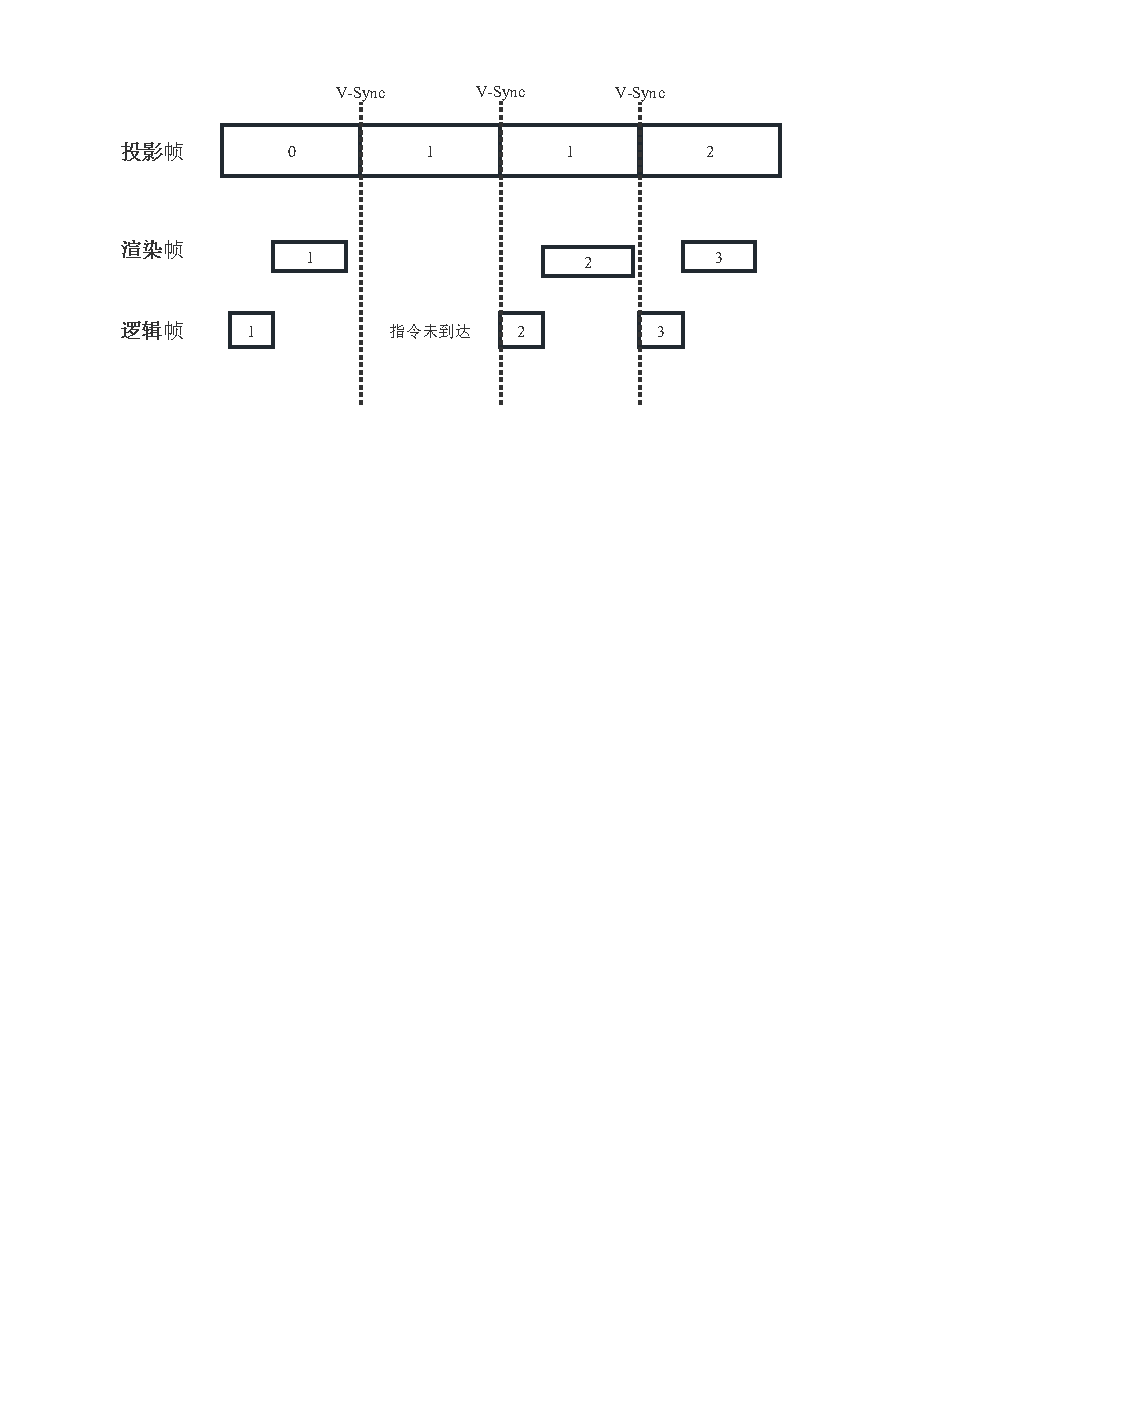
\includegraphics[width=\textwidth]{pictures/tearreason.pdf}
        \caption{画面撕裂情况}
        \label{tearreason}
    \end{center}
\end{figure}
\par 
接下来就需要排查指令不能及时到达图像生成器的原因。前面提到机房的网络环境十分优秀,网络波动基本可以排除。
从整个指令流动过程可知,可能令指令到达频率不稳定的地方有二,一是虚拟仿真机接收仿真机指令的频率不稳定,二是发送给多台图像生成器时存在时间上的差距。
其中
\subsection{网络帧缓冲}
\section{数据平滑机制}
\subsection{问题分析}
加入数据帧缓冲机制后,画面撕裂和顿挫现象基本消失,三台图像生成器可以同时使用同一帧的数据进行计算,
而且屏蔽了由于虚拟仿真机接收数据的频率不稳定而导致的时延。但又发现单一图像生成器产生的画面会沿飞机运动方向产生抖动。
从数据角度来看可能的原因是数据精度不够或者数据变化不平滑。
\begin{figure}[h!]
    \begin{center}
        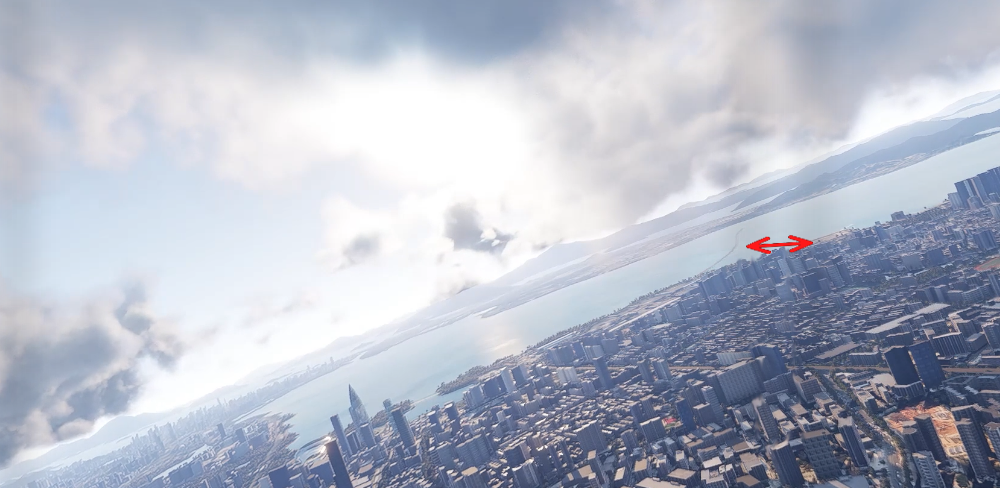
\includegraphics[width=\textwidth]{pictures/jitter.png}
        \caption{画面抖动情况}
        \label{jitter}
    \end{center}
\end{figure}
\subsection{插值平滑}
\par
系统测试是为了在用户开始使用软件前,尽可能地发现软件中潜在的错误
和不合理之处,确保最后将高质量的软件交付给用户。为了验证系统的功能和
性能是否与需求分析时的规格说明一致,本章节在开发环境和真实FFS环境中分别做综合性的功能测试和性能测试。

在第二章的介绍中提到Nagle算法可以减少TCP包的个数,更高效的利用网络带宽。但同时也会带来一些延时问题,在实时交互应用中尤其重要。
对于部署虚拟仿真机和游戏引擎的Windows系统机器都需要在注册表中将TcpAckFrequency字段和TcpNoDelay字段值修改为1,以禁用Nagle算法。
\begin{figure}[h!]
    \begin{center}
        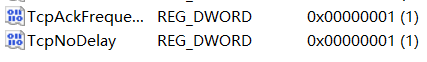
\includegraphics[width=0.8\textwidth]{pictures/nagle.png}
        \caption{Windows中禁用Nagle}
    \end{center}
\end{figure}
\section{开发PC环境测试}
由于国内的FFS全部位于航空公司的训练基地内,不具备移动的可能性,平日开发过程中的测试均使用虚拟仿真机读取模拟数据,并在开发PC上完成视景渲染。
受限于硬件性能,在开发环境下的测试以功能测试为主,确保功能正常运作即可,对于画面帧率和分辨率之类不做严格要求。
\subsection{测试环境}
在开发环境下,虚拟仿真机由笔记本电脑担任,模拟数据也位于该电脑上,在Windows系统上运行程序,便可以通过Tbuspp与视景建立连接,不断地读取并发送数据。
对于运行视景的机器有较高的硬件要求,GPU部分要使用较高型号才能让开发人员流畅的观察场景。同时由于搭载了大型机场场景数据库,对于硬盘容量也有较高要求。在测试环境的具体物理配置信息如表\ref{devhard}所示。
\begin{table}[h!]
    \begin{center}
        \caption{开发环境物理配置}
        \renewcommand\arraystretch{1.5}
        \label{devhard}
        \begin{tabularx}{\textwidth}{ 
             >{\centering\arraybackslash\hsize=.4\hsize\linewidth=\hsize}X 
             >{\centering\arraybackslash\hsize=.4\hsize\linewidth=\hsize}X 
             >{\centering\arraybackslash\hsize=\hsize\linewidth=\hsize}X 
             }
             \hline
            \textbf{设备} & \textbf{配置项} & \textbf{详情}\\
             \hline
             & CPU & AMD Ryzen 7 4700G 8-Core Processor\\
           
             & GPU & NVIDIA GeForce RTX 3060\\
             
             视景运行机 & 内存 & 32GB\\
            
             & 硬盘 & 8TB\\
             
             & 系统 & Windows 10 专业版 22H2\\
             \hline
             & CPU & AMD Ryzen 7 5800H with Radeon Graphics\\
           
             & GPU & AMD Radeon(TM) Graphics\\
             
             虚拟仿真机 & 内存 & 16GB\\
            
             & 硬盘 & 512GB\\
             
             & 系统 & Windows 10 专业版 22H2\\
             \hline
            \end{tabularx}
    \end{center}
\end{table}
\par

\subsection{功能测试}

我们在测试中使用到的模拟数据是飞行员在训练基地FFS上操作绕深圳宝安机场飞行一周后得到的数据。
该数据的采样频率为60Hz,共6万余组数据,每组数据中包含仿真机输出的原始经纬高和欧拉角信息。
首先测试经过虚拟仿真机发送给游戏引擎的数据是否正确,采用的方法是在GIS软件中绘制这组输出数据,查看绘制路径与飞行员的飞行路径是否相同。
图\ref{GIStrace}中的轨迹是由上述原始数据经过虚拟仿真机处理最终输出的6万个点构成,可以看到轨迹起始位置精确的位于宝安机场的跑道上,
起飞后环绕深圳市区飞行,最终截止于羊台山森林公园。与飞行员核对后确认本路径准确无误,说明由仿真机到游戏引擎中间一系列数据操作均可以通过测试。

\par
在确认虚拟仿真机输出无误后,便可使用此数据进一步测试游戏引擎中飞行控制逻辑。图\ref{firsttest}是飞机第一视角下的飞行画面,可以看到根据模拟数据,飞机准确出现在宝安机场跑道上,
且后续飞行中的爬升转向时的视角偏转完全符合实际情况,最终飞机按照轨迹终止于场景中的森林公园上空。此测试过程同样表明第一视角摄像机可以正确跟随飞机位置并做出相同的姿态。



\par
当摄像机位于第一视角下,按下X键即可切换为环绕视角。如图\ref{orbittest}所示,此时摄像机不在位于驾驶舱位置,而是在一定距离外始终看向驾驶舱。
鼠标左右方向的滑动可以改变Yaw角使摄像机水平方向的环绕,上下的滑动则改变Pitch角是竖直方向的环绕。经测试操作感受与主流游戏基本一致。

\begin{figure}[h!]
    \begin{center}
        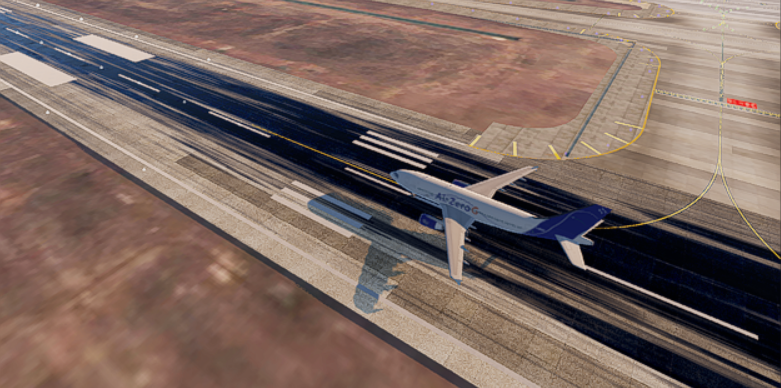
\includegraphics[width=0.9\textwidth]{pictures/orbitcamera.png}
        \caption{飞机环绕视角}
        \label{orbittest}
    \end{center}
\end{figure}
\par
当摄像机位于环绕视角下,按下X键即可切换为自由视角。如图\ref{freetest}所示,此时摄像机会在当前位置脱离飞机,并可以去到场景中的任意位置。
键盘的WASD键为前后左右移动,EQ键控制上下移动,这些移动方向都根据摄像机自身坐标系改变。Shift键则可以加速移动。经测试,操作感受与游戏引擎中的场景漫游基本一致。
\begin{figure}[h!]
    \begin{center}
        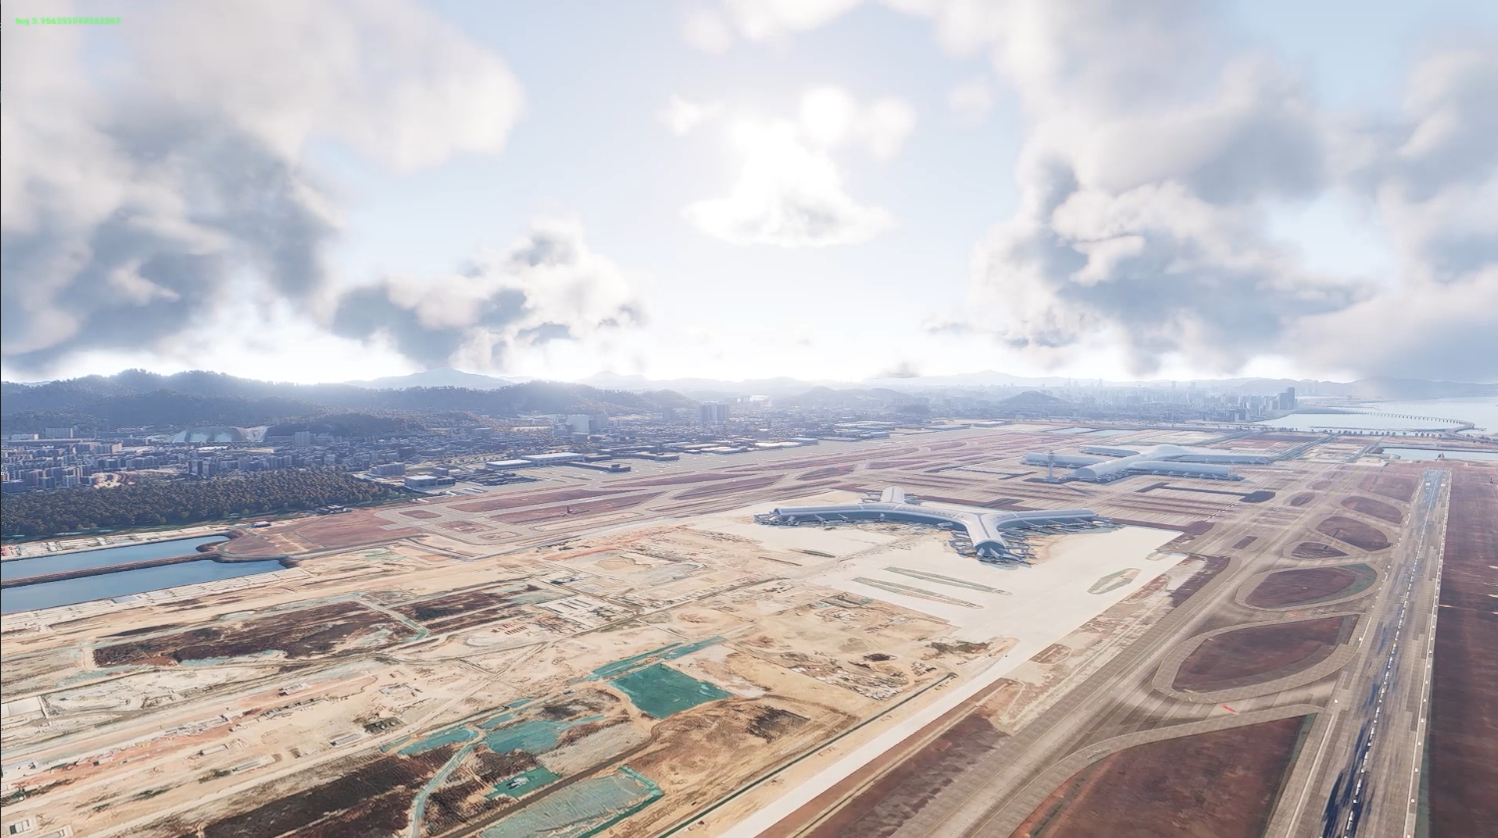
\includegraphics[width=.85\textwidth]{pictures/freecamera.png}
        \caption{自由视角}
        \label{freetest}
    \end{center}
\end{figure}


\subsection{功能测试}
仿真机与虚拟仿真机通过网线连接。测试中启动与仿真机连接程序后,先选择要使用的网卡。连接建立成功后便可以开始正常接收数据。测试情况如图\ref{vsimcon}所示。
虚拟仿真机已成功读取到网卡上来自仿真机的原始数据包。
\par
对于数据交换相关用例的测试同样是与服役中的FFS使用同一条预设路径飞行进行对比。本次测试选择的机场为广州白云机场,路径为跑道上的起飞过程。在服役FFS中运行的视频效果如图\ref{flightffs}所示,飞机即将在白云机场02L号跑道上完成起飞。
图\ref{flightffs}则展示了本视景系统运行该路径的情况,系统可以根据仿真机的数据正确将飞机初始位置置于机场02L号跑道,且在后续起飞过程中视景画面与上述服役FFS视频中完全一致。
目前画面仍存在球幕上的畸变问题以及颜色不准确的问题,但对于数据交换系统而言已经实现了核心功能。
\begin{figure}[h!]
    \begin{center}
        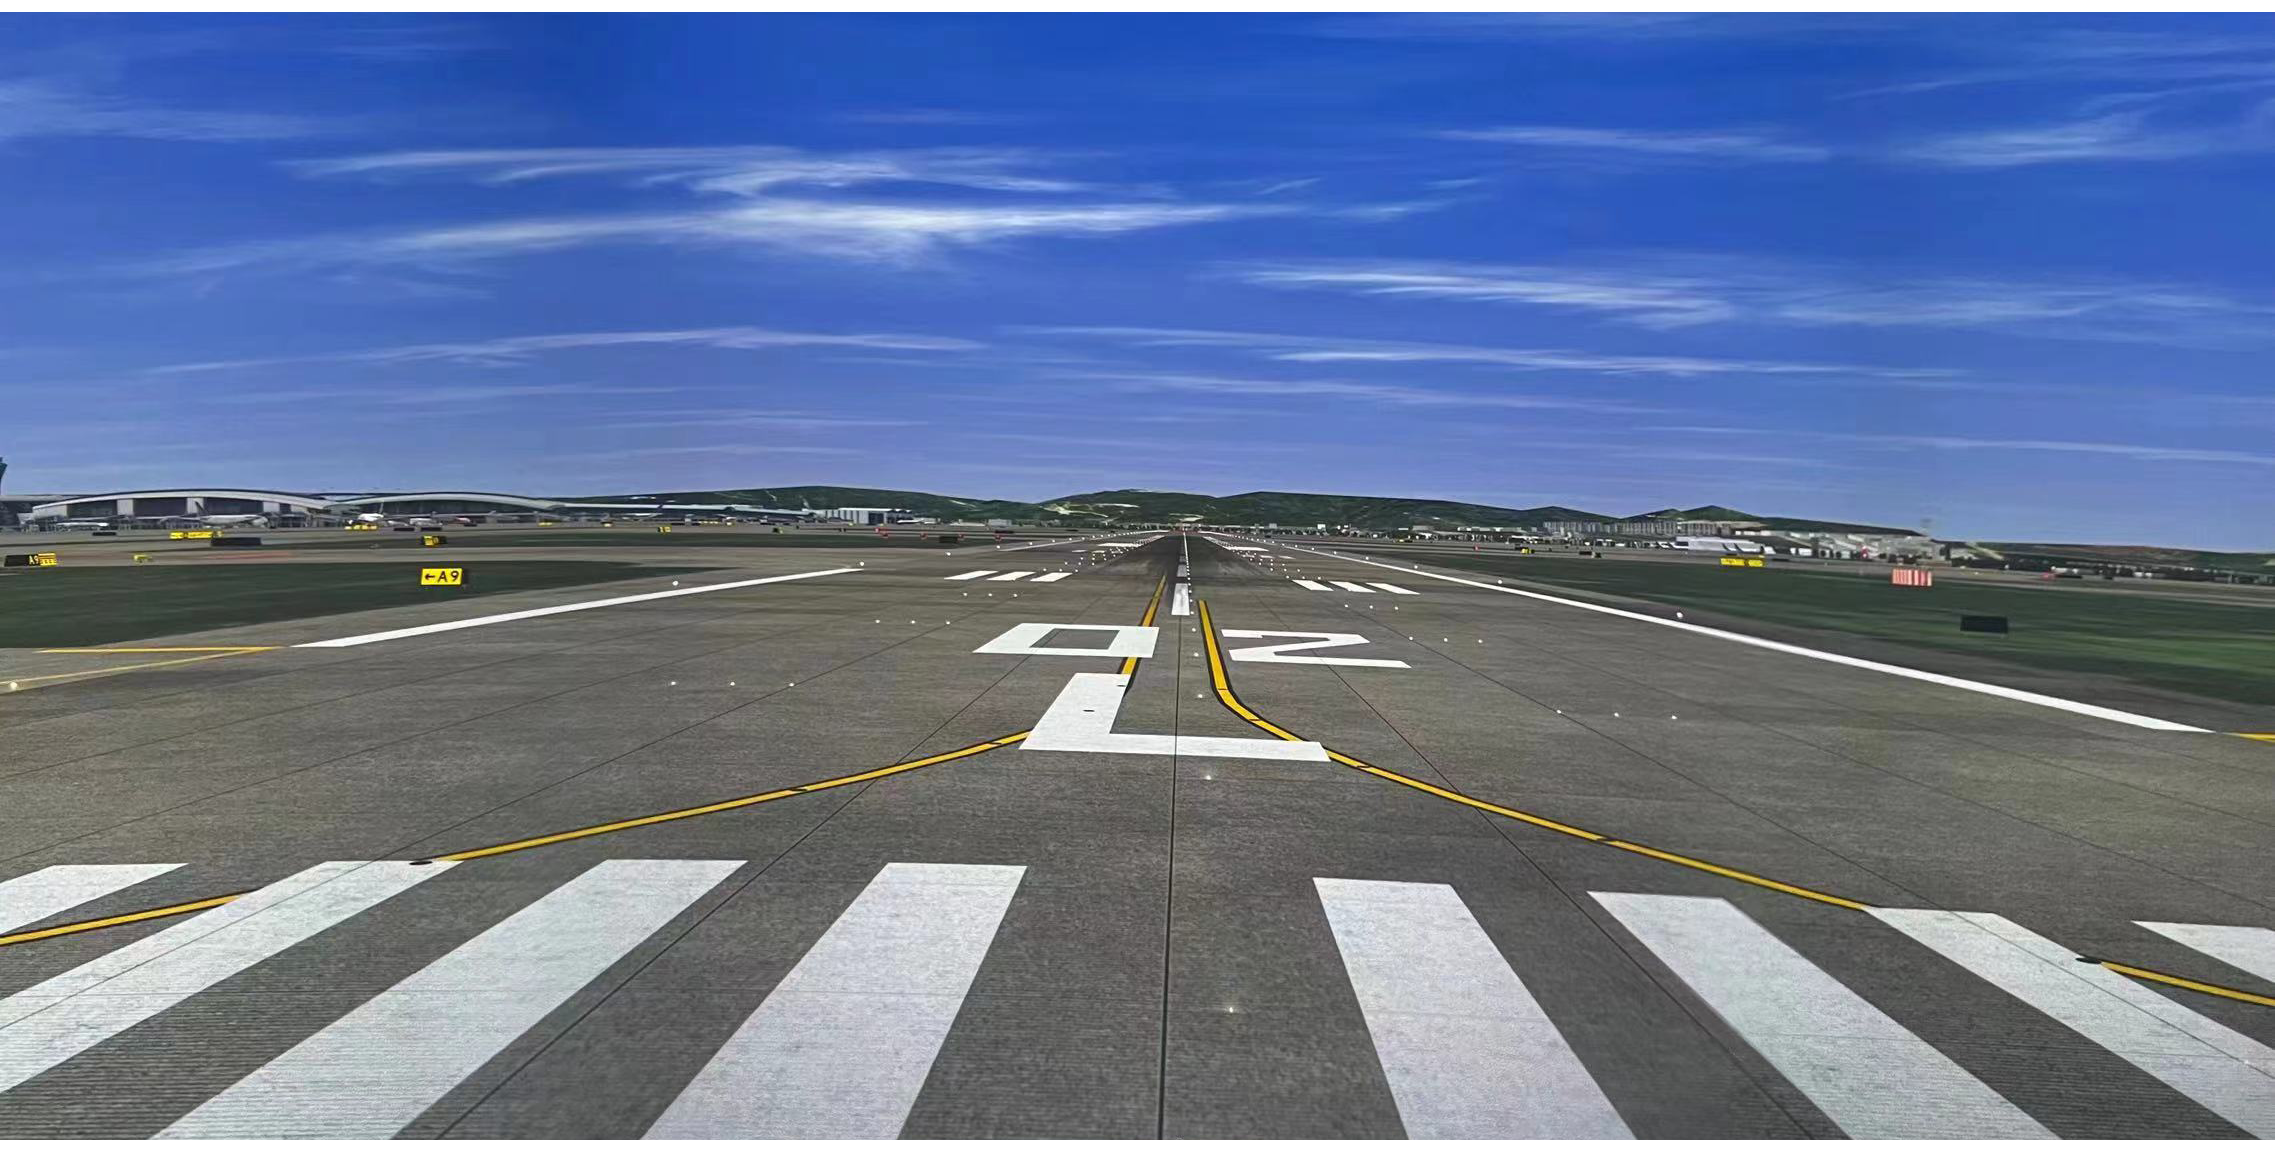
\includegraphics[width=.8\textwidth]{pictures/ffs2.png}
        \caption{服役中FFS运行效果}
        \label{flightffs}
    \end{center}
\end{figure}
\begin{figure}[h!]
    \begin{center}
        \includegraphics[width=.8\textwidth]{pictures/ffs.png}
        \caption{本视景系统运行舱内效果}
        \label{flighttest}
    \end{center}
\end{figure}
\subsection{性能测试}
性能测试的部分主要测试连续运行下视景系统的帧率稳定性。帧率检测使用第三方的监控软件,连续飞行一个小时,记录平均帧率、最高帧率、最低帧率和1\% Low帧的情况。
其中最高帧率与最低帧率并不是某一时刻的帧率,而是极短时间内的平均帧率。1\% Low是选取了帧生成时间最长的1\%的帧计算的平均帧率,这些帧不一定是连续的,所以一般会低于最低帧率,
表示整段测试时间内某些时刻的剧烈帧率波动。
\par
测试结果如表\ref{frametest}所示,视景系统限制帧率上限为60FPS,平均帧率十分接近这一数值,说明总体来讲基本能达到长时间运行下的帧率要求。
最高帧率60.8FPS说明对于帧率的限制较为成功。1\%Low距离平均帧率有较大的距离,说明在某些复杂场景下会产生比较剧烈的瞬时帧率波动。
\begin{table}[h!]
    \begin{center}
        \caption{帧率测试结果表}
        \label{frametest}
        \renewcommand\arraystretch{1.5}
        \begin{tabularx}{0.8\textwidth}{ 
             |>{\centering\arraybackslash\hsize=\hsize\linewidth=\hsize}X 
             |>{\centering\arraybackslash\hsize=\hsize\linewidth=\hsize}X 
             |
             }
             \hline 
            \textbf{项目} & \textbf{数值}\\   
             \hline
             运行时间 & 3612.015s\\
             \hline
             总帧数 & 212748 Frame\\     
             \hline
             平均帧率 & 58.9 FPS\\
             \hline 
             最低帧率& 48.6 FPS\\
             \hline 
             最高帧率& 60.8 FPS\\
             \hline 
             1\% Low& 28.1 FPS\\
             \hline  
            \end{tabularx}
    \end{center}
\end{table}
\section{系统测试}
\section{本章小结}
本章首先介绍了系统测试,通过系统测试可以有效保证系统的质量,同时可以验证系统的可用性。
随后将测试分为了开发环境和真实FFS环境,分别作了部分功能测试,并由于硬件性能原因只在FFS环境中做了性能测试。
通过此测试可以证明系统满足需求分析中的功能需求,并在FFS环境中达成非功能需求。